\documentclass[final,hyperref={pdfpagelabels=false}]{beamer}
\mode<presentation>{\usetheme{edf}}
  %\usepackage{times}
  \usepackage{ragged2e} %% justify the text.
  \usepackage{amsmath,amsthm, amssymb, latexsym}
  %\boldmath
  \usepackage[english]{babel}
  \usepackage[utf8]{inputenc}

\usepackage{graphicx}
\graphicspath{{img/}}

\usepackage{subfigure}


% \usepackage[orientation=portrait,size=custom,width=40,height=80,scale=.6,debug]{beamerposter}
  \usepackage[orientation=portrait,size=a0,scale=1]{beamerposter} %% this can scale the entire poster to make it smaller or bigger.



\usepackage[absolute,overlay]{textpos}
\usepackage{subfigure}



%\usefonttheme{professionalfonts}
%\usefonttheme{serif}
%\usepackage{fontspec}
%\setmainfont{Avenir}

\TPGrid[0mm,0mm]{80}{60}







%-- Header and footer information ----------------------------------
\newcommand{\footleft}{EDF Lab\\Centre R\& D des Renardières}
\newcommand{\footright}{email: mail@mvkonnik.info}
\title{Compatible Susceptibility Measurements\\ in Fully Anechoic Room and Reverberation Chamber}
\author{E. Amador, C. Miry and N. Bouyge}
\institute{LME, EDF Lab, les Renardières, France.\\[0.5cm]\Large{\texttt{emmanuel.amador@edf.fr}}}

%-------------------------------------------------------------------


%-- Main Document --------------------------------------------------
\begin{document}

\begin{textblock}{14}(1.5,0.75)
\includegraphics[trim=0 0 0 0,clip,scale=.9]{./img/EDF_LOGO_blanc}
\end{textblock}

\begin{textblock}{14}(66.3,1.45)
\includegraphics[trim=0 0 0 0,clip,scale=.8]{./img/EDFLAB_LOGO_blanc}
\end{textblock}

\begin{textblock}{0.1}(26.65,8.7)
\vrule width 1pt height 86cm
\end{textblock}

\begin{textblock}{0.1}(52.95,8.7)
\vrule width 1pt height 86cm
\end{textblock}

\begin{frame}{}

      \begin{block}{\huge{Summary}}
      \LARGE{By considering that an \textbf{immunity testing is a binomial process}~\cite{Amador13}, measurements performed with deterministic fields like a fully anechoic room (FAR) and measurements performed with random fields like a reverberation chamber (RC) can give very similar values.}  
      \end{block}
% \hrule
  \begin{columns}[t]
% 
%     %-- Column 1 ---------------------------------------------------
    \begin{column}{0.32\linewidth}

      %-- Block 1-1
	\vspace{-1cm}
      \begin{block}{Motivation}  \justifying
       \large{The comparison of testing facilities is a subject of interest in the EMC community.
	 The confidence intervals (generally $\pm 3~dB$) provided by standard measurements~\cite{IEC21,IEC22} does not allow a good agreement between the measurements.

      }
\end{block}
\begin{center}\begin{minipage}{0.9\textwidth}
	\begin{exampleblock}{{Solution}} \justifying
  \large{If the susceptibility of a device is a random variable, we can develop a \textbf{common statistical framework} to extract with a controlled uncertainty the susceptibility levels of the equipments tested in our lab. }
	\end{exampleblock}
\end{minipage}\end{center}
      %-- Block 1-2
      \begin{block}{{Statistical characterization of the susceptibility of a non-intentional emitter}} \justifying
        \large{ In order to extract the statistics of the E-field radiated by a non-intentional emitter, we use a model of non intentional emitter used by P.~Wilson~\cite{Wilson02}. $n$ random Hertz dipoles are placed arbitrary on a sphere of radius $a$.\\
We study the effects of the complexity (number of dipoles $n$) and the electrical size $ka=\frac{2\pi}{\lambda}a$ on the statistics of the radiated E-field.


\vspace{-0.6cm}
\begin{figure}
\includegraphics[trim=70 70 70 60,clip,width=0.3\columnwidth]{./img/eut}
\vspace{-0.3cm}
\large{\caption{A non-intentional emitter}}
\end{figure}}

\vspace{-0.6cm}
\begin{figure}
     \centering
     \subfigure[$f=20$ MHz, $ka=0.4$, $D\approx 1.6$]{
          \label{fig_800M}      
          \includegraphics[trim=110 180 90 120,clip,width=0.45\columnwidth]{./img/rp_4.png}} 
    \subfigure[$f=100$ MHz, $ka=2.1$, $D\approx 2.3$]{
          \label{fig_2G}
   	  \includegraphics[trim=110 170 90 120,clip,width=0.45\columnwidth]{./img/rp_24.png}}\\
\subfigure[$f=500$ MHz, $ka=10.5$, $D\approx 5.2$]{
             \label{fig_800M}      
          \includegraphics[trim=110 180 90 120,clip,width=0.45\columnwidth]{./img/rp_124.png}} 
    \subfigure[$f=1000$ MHz, $ka=21.0$, $D\approx 5.7$]{
          \label{fig_2G}
          \includegraphics[trim=110 180 90 120,clip,width=0.45\columnwidth]{./img/rp_249.png}}
\vspace{-0.3cm}
    \large{\caption{Radiated power (linear values) of a random EUT with  $a=1$ m and $n=100$ dipoles}}
     \label{fig_diagsr}
\end{figure}
Monte Carlo simulations give an idea of the statistics of the E-field rectangular components radiated by such emitters:
%\vspace{0.6cm}
\begin{figure}
     \centering
     \subfigure[$ka=1$, $n=4$]{
          \label{fig_800M}      
          \includegraphics[trim=20 20 20 10,width=0.44\columnwidth]{./img/CDF_ka_1_n_4.png}} 
    \subfigure[$ka=2$, $n=4$]{
          \label{fig_2G}
   	  \includegraphics[trim=20 20 20 10,width=0.44\columnwidth]{./img/CDF_ka_2_n_4.png}}\\
\subfigure[$ka=3$, $n=4$]{
             \label{fig_800M}      
         \includegraphics[trim=20 20 20 10,width=0.44\columnwidth]{./img/CDF_ka_3_n_4.png}} 
    \subfigure[$ka=10$, $n=10$]{
          \label{fig_2G}
          \includegraphics[trim=20 20 20 10,width=0.44\columnwidth]{./img/CDF_ka_10_n_10.png}}
\vspace{-0.3cm}
    \large{\caption{Cumulative distribution functions of the E-field rectangular components vs. theoretical Rayleigh distribution}}
     \label{fig_diagsr}
\end{figure}
\end{block}

     

    \end{column}%1

    %-- Column 2 ---------------------------------------------------
    \begin{column}{0.32\linewidth}
\vspace{-1cm}
%Anderson-Darling statistical test gives the probability to get a Rayleigh distribution for every combination of $n$ and $ka$:
\vspace{-0.6cm}
\begin{figure}
\centering
\includegraphics[trim=0 0 0 0,clip,width=0.7\columnwidth]{./img/TestAD}
\vspace{-0.3cm}
\large{\caption{Probability to get a Rayleigh distributed E-field component according to the Anderson-Darling statistical test, $10^5$ Monte Carlo trials for every point}}
\end{figure}

      %-- Block 2-1
 \begin{block}{Statistical estimation of the susceptibility}
\vspace{-0.6cm}
\begin{figure}
\centering
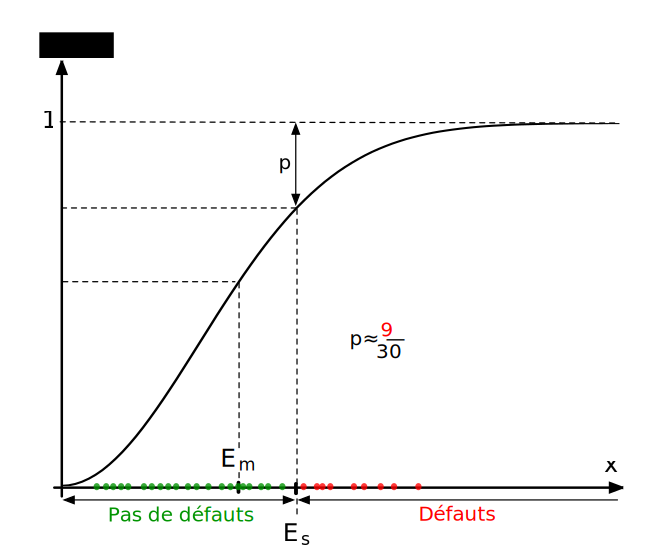
\includegraphics[trim=0 0 0 0,clip,width=0.8\columnwidth]{./img/rayleighCDF}
\vspace{-0.3cm}
\large{\caption{Statistical estimation of the susceptibility $E_s$ \cite{Amador13} of an EUT if the impinging E-field components follows a Rayleigh distribution with mean value $E_m$.}}
\end{figure}
\large{
\begin{equation*}
\hat{E}_s=2E_m\sqrt{\frac{\ln(1/\hat{p})}{\pi}}
\end{equation*}}


\vspace{-0.6cm}
\begin{figure}
\centering
\includegraphics[trim=0 0 0 0,clip,width=0.8\columnwidth]{./img/figErrbc}
\vspace{-0.3cm}
\large{\caption{Confidence intervals of $\hat{E}_s$.}}
\end{figure}
      \end{block}

      %-- Block 2-2

      \begin{block}{A generic EUT}
\vspace{-0.6cm}
      \begin{figure}
     \centering
     \subfigure[]{
          \label{fig_800}      
          \includegraphics[width=.48\columnwidth]{./img/EUT_ext.png}} 
    \subfigure[]{
          \label{fig_2000}
          \includegraphics[width=.48\columnwidth]{./img/EUT_int.png}}
     \vspace{-0.3cm}
\large{\caption{External (a) and internal (b) views of the generic EUT.}}
     \label{fig_diags}
\end{figure}
\vspace{-0.2cm}
\centering{\textit{``If the level on the $z$ axis exceeds the critical value $E_c=10$~V/m, we consider that the EUT exhibits a failure.''}}

\vspace{-0.6cm}
\begin{figure}
     \centering
     \subfigure[800~MHz]{
          \label{fig_800}      
          \includegraphics[trim=220 220 220 220,clip,width=.31\columnwidth]{./img/ka_800_44.png}} 
    \subfigure[ 2~GHz]{
          \label{fig_2000}
          \includegraphics[trim=220 220 220 220,clip,width=.31\columnwidth]{./img/ka_2000_36.png}}
    \subfigure[4~GHz]{
          \label{fig_4000}
          \includegraphics[trim=270 270 270 270,clip,width=.31\columnwidth]{./img/ka_4000_12.png}}
     \vspace{-0.3cm}
\large{\caption{Radiation patterns at different frequencies (CST simulations).}}
     \label{fig_diagsCST}
\end{figure}
\end{block}
      %-- Block 2-3
     

    \end{column}%2

    %-- Column 3 ---------------------------------------------------
    \begin{column}{0.32\linewidth}

\vspace{-1.0cm}
 \begin{block}{Measurements}
       \large{ \begin{itemize}
	\item Measurements are performed between 800~MHz and 4~GHz
	\item Calibration of the RC and the FAR is done for \textbf{every} frequency tested
	\item $n$ angles of incidence are randomly chosen for the FAR measurement. $n$ stirrer positions in the RC
	\item Tested levels $E_m$ are 5, 10 , 20, 40, 80 V/m. 
	\end{itemize}}
      \end{block}
%\vspace{-1.5cm}
      %-- Block 3-1
      \begin{block}{Results}
\vspace{-0.5cm}
\begin{figure}
     \centering
     \subfigure[]{
          \label{fig_800}      
          \includegraphics[trim=10 13 00 15,clip,width=.85\columnwidth]{./img/mesures_apres}}\\
    \subfigure[]{
          \label{fig_2000}
          \includegraphics[trim=10 00 00 15,clip,width=.85\columnwidth]{./img/mesures_bpres}}
     \vspace{-0.3cm}
\large{\caption{Susceptibility measurement with $n=30$ observations.}}
     \label{fig_diagsCST}
\end{figure}
\vspace{-0.6cm}
\begin{figure}
     \centering
     \subfigure[]{
          \label{fig_800}      
          \includegraphics[trim=10 13 00 15,clip,width=.85\columnwidth]{./img/mesures_a10pres}}\\
    \subfigure[]{
          \label{fig_2000}
          \includegraphics[trim=10 00 00 15,clip,width=.85\columnwidth]{./img/mesures_b10pres}}
     \vspace{-0.3cm}
\large{\caption{Susceptibility measurement with $n=10$ observations.}}
     \label{fig_diagsCST}
\end{figure}
\vspace{0.8cm}
\large{As long as the EUT is electrically large enough:
\begin{itemize}
\item Good agreement of the measurements
\item With $n=10$, the agreement is good enough for EMC purpose
\end{itemize}}
      \end{block}
    \end{column}%3
  \end{columns}

\begin{block}{\Huge{Conclusion}} \justifying
\Large{By using a common statistical framework for both the FAR and the RC and as long as the EUT is electrically large and complex, we can extract with a good agreement the immunity levels of an EUT. By giving a statistical dimension to FAR measurements, we can control and enhance the accuracy of the measurement.}
	\end{block}%-- Block 1-2


\begin{columns}
%     %-- Column 1 ---------------------------------------------------

 \begin{column}{0.71\linewidth}
\vspace{-0.3cm}   
\begin{block}{References} \justifying
\setbeamertemplate{bibliography item}[text]
\setbeamercolor{bibliography item}{fg=black,bg=white}
\setbeamercolor{bibliography entry author}{fg=black,bg=white}
\setbeamercolor{bibliography item}{fg=black,bg=white}
\bibliographystyle{IEEEtran}
 \small
\bibliography{IEEEabrv,biblio}
	\end{block}

    \end{column}%1

    %-- Column 2 ---------------------------------------------------
    \begin{column}{0.2\linewidth}
    \vspace{-0.4cm}
  \begin{block}{Acknowledgments}
    \vspace{-0.5cm}
Measurements and simulations made with:\\\centerline{\includegraphics[trim=150 120 120 60,clip,width=.3\columnwidth]{./img/python_logo.png}
\hspace{1cm} \includegraphics[width=.15\columnwidth]{./img/julia.png}}
Poster, data, scripts available at:\\\href{https://github.com/manuamador/EMCEurope2014}{\small{\texttt{https://github.com/manuamador/EMCEurope2014}}}
      \end{block}
\end{column}%2
 %-- Column 2 ---------------------------------------------------
\begin{column}{0.07\linewidth}

\end{column}%2
  \end{columns}
\begin{textblock}{14}(73.2,56.5)
\includegraphics[trim=40 40 40 40,clip,scale=.52]{./img/QR.png}
\end{textblock}
\end{frame}
\end{document}